\documentclass[10pt]{extarticle}
\title{}
\author{Avinash Iyer}
\date{}
\usepackage[shortlabels]{enumitem}

%font setup
%
\usepackage{newpxtext,eulerpx}

%paper setup
\usepackage{geometry}
\geometry{letterpaper, portrait, margin=1in}
\usepackage{fancyhdr}

%symbols
\usepackage{amsmath}
\usepackage{mathtools}
\usepackage{hyperref}
\usepackage{gensymb}

\usepackage[T1]{fontenc}
\usepackage[utf8]{inputenc}

\usepackage[version=4]{mhchem}
\usepackage{chemfig}

%plotting
\usepackage{pgfplots}
\usepackage{tikz}
\tikzset{middleweight/.style={pos = 0.5, fill=white}}
\tikzset{weight/.style={pos = 0.5, fill = white}}
\tikzset{lateweight/.style={pos = 0.75, fill = white}}
\tikzset{earlyweight/.style={pos = 0.25, fill=white}}

%\usepackage{natbib}

%graphics stuff
\usepackage{graphicx}
\graphicspath{ {./images/} }

%code stuff
%when using minted, make sure to add the -shell-escape flag
%you can use lstlisting if you don't want to use minted
%\usepackage{minted}
%\usemintedstyle{pastie}
%\newminted[javacode]{java}{frame=lines,framesep=2mm,linenos=true,fontsize=\footnotesize,tabsize=3,autogobble,}
%\newminted[cppcode]{cpp}{frame=lines,framesep=2mm,linenos=true,fontsize=\footnotesize,tabsize=3,autogobble,}

\usepackage{listings}
\usepackage{color}
\definecolor{dkgreen}{rgb}{0,0.6,0}
\definecolor{gray}{rgb}{0.5,0.5,0.5}
\definecolor{mauve}{rgb}{0.58,0,0.82}

\lstset{frame=tb,
	language=Java,
	aboveskip=3mm,
	belowskip=3mm,
	showstringspaces=false,
	columns=flexible,
	basicstyle={\small\ttfamily},
	numbers=none,
	numberstyle=\tiny\color{gray},
	keywordstyle=\color{blue},
	commentstyle=\color{dkgreen},
	stringstyle=\color{mauve},
	breaklines=true,
	breakatwhitespace=true,
	tabsize=3
}
% text + color boxes
\usepackage[most]{tcolorbox}
\tcbuselibrary{breakable}
\newtcolorbox{problem}[1]{colback = white, title = {#1}, breakable}
\newtcolorbox{solution}{colback = white, colframe = black!75!white, title = Solution, breakable}
%including PDFs
\usepackage{pdfpages}
\setlength{\parindent}{0pt}

\pagestyle{fancy}
\fancyhf{}
\rhead{Avinash Iyer}
\lhead{Econ 308: Class Notes}
\begin{document}
  \begin{problem}{Introduction to Public Economics}
    Governments play a crucial role in much economic life.
    \begin{itemize}
      \item Regulatory structure (financial markets, pharmaceuticals, labor markets, civil rights).
      \item Taxes.
      \item Public goods and social welfare spending.
      \item Macroeconomic stabilization.
    \end{itemize}
   Public finance is the study of the role of government in a market economy, primarily focusing on taxes and spending.\\

   Reasons to study public economics:
    \begin{itemize}
      \item Governments have a lot of power in the realm of economic welfare.
      \item Nearly every economic transition is mediated by the government.
      \item It can inform debates about the appropriate role of government regarding taxes, healthcare, climate change, etc.
      \item The government is large.
        \begin{itemize}
          \item It employs 1/6 of the US Workforce.
          \item Tax revenue is approximately 27\% of the United States's Gross Domestic Product.
        \end{itemize}
    \end{itemize}
    The government (as measured by tax revenue/GDP) greatly increased in size between 1910 and 1940 (due to the establishment of the welfare state and various wars).
    \begin{center}
      \begin{tikzpicture}
            \begin{axis}[
                title = {Federal Spending (red) and Tax Receipts (blue) as a proportion of GDP},
                xlabel = {Year},
                ylabel = {Percentage of GDP},
               y tick label style={/pgf/number format/.cd,%
            scaled y ticks = false,
            set thousands separator={},
            fixed}, xmin = 1929, xmax = 2022,
                x tick label style={/pgf/number format/.cd,%
            scaled y ticks = false,
            set thousands separator={},
            fixed},ymin = 0, ymax = 45,
                ytick = {0,5,10,15,20,25,30,35,40,45},
              width=\textwidth,
              axis lines = left,height=\axisdefaultheight
              ]
               \addplot[color=blue] table[x index=0, y index=1]{receipts_expenditures.tsv};
               \addplot[color=red] table[x index=0, y index=2]{receipts_expenditures.tsv};
            \end{axis}
    \end{tikzpicture}
    \end{center}
    \begin{problem}{Two Motivations for Government Intervention}
      \begin{itemize}
        \item Market Failure
        \item Redistribution
      \end{itemize}
      The First Welfare Theorem states that \textit{in the absence of market failure}, markets will yield a result along the \textbf{utility possibilities frontier} (i.e., the set of all maximized utilities given the current market).

      However, there are a lot of market failures:
      \begin{itemize}
        \item Externalities (pollution, network effects from vaccination)
        \item Public Goods (public safety)
        \item Asymmetric Information (market for lemons)
        \item Individual Mistakes (failure to save)
        \item Imperfect Competition (oligopoly, cartelization)
      \end{itemize}
      Policymakers also have to consider the \textit{equity-efficiency tradeoff} in redistribution (i.e., some redistributive acts might reduce total utility)
    \end{problem}
    \begin{problem}{Government as Social Cooperation}
      \begin{itemize}
        \item Economists tend to have a narrow view of human behavior, but social cooperation undergirds much of the levels of societal coordination beyond individuals (i.e., families, communities, countries, global superstructures)
        \item Human societies of old depended on social cooperation for protection and taking care of the young, sick, and old.
        \item Modern states are the primary form of coordination today.
        \item Humans reveal their social nature (or social solidarity) via the size of the government (informal and formal).
      \end{itemize}
    \end{problem}
    \begin{problem}{Activity 1}
      \begin{center}
        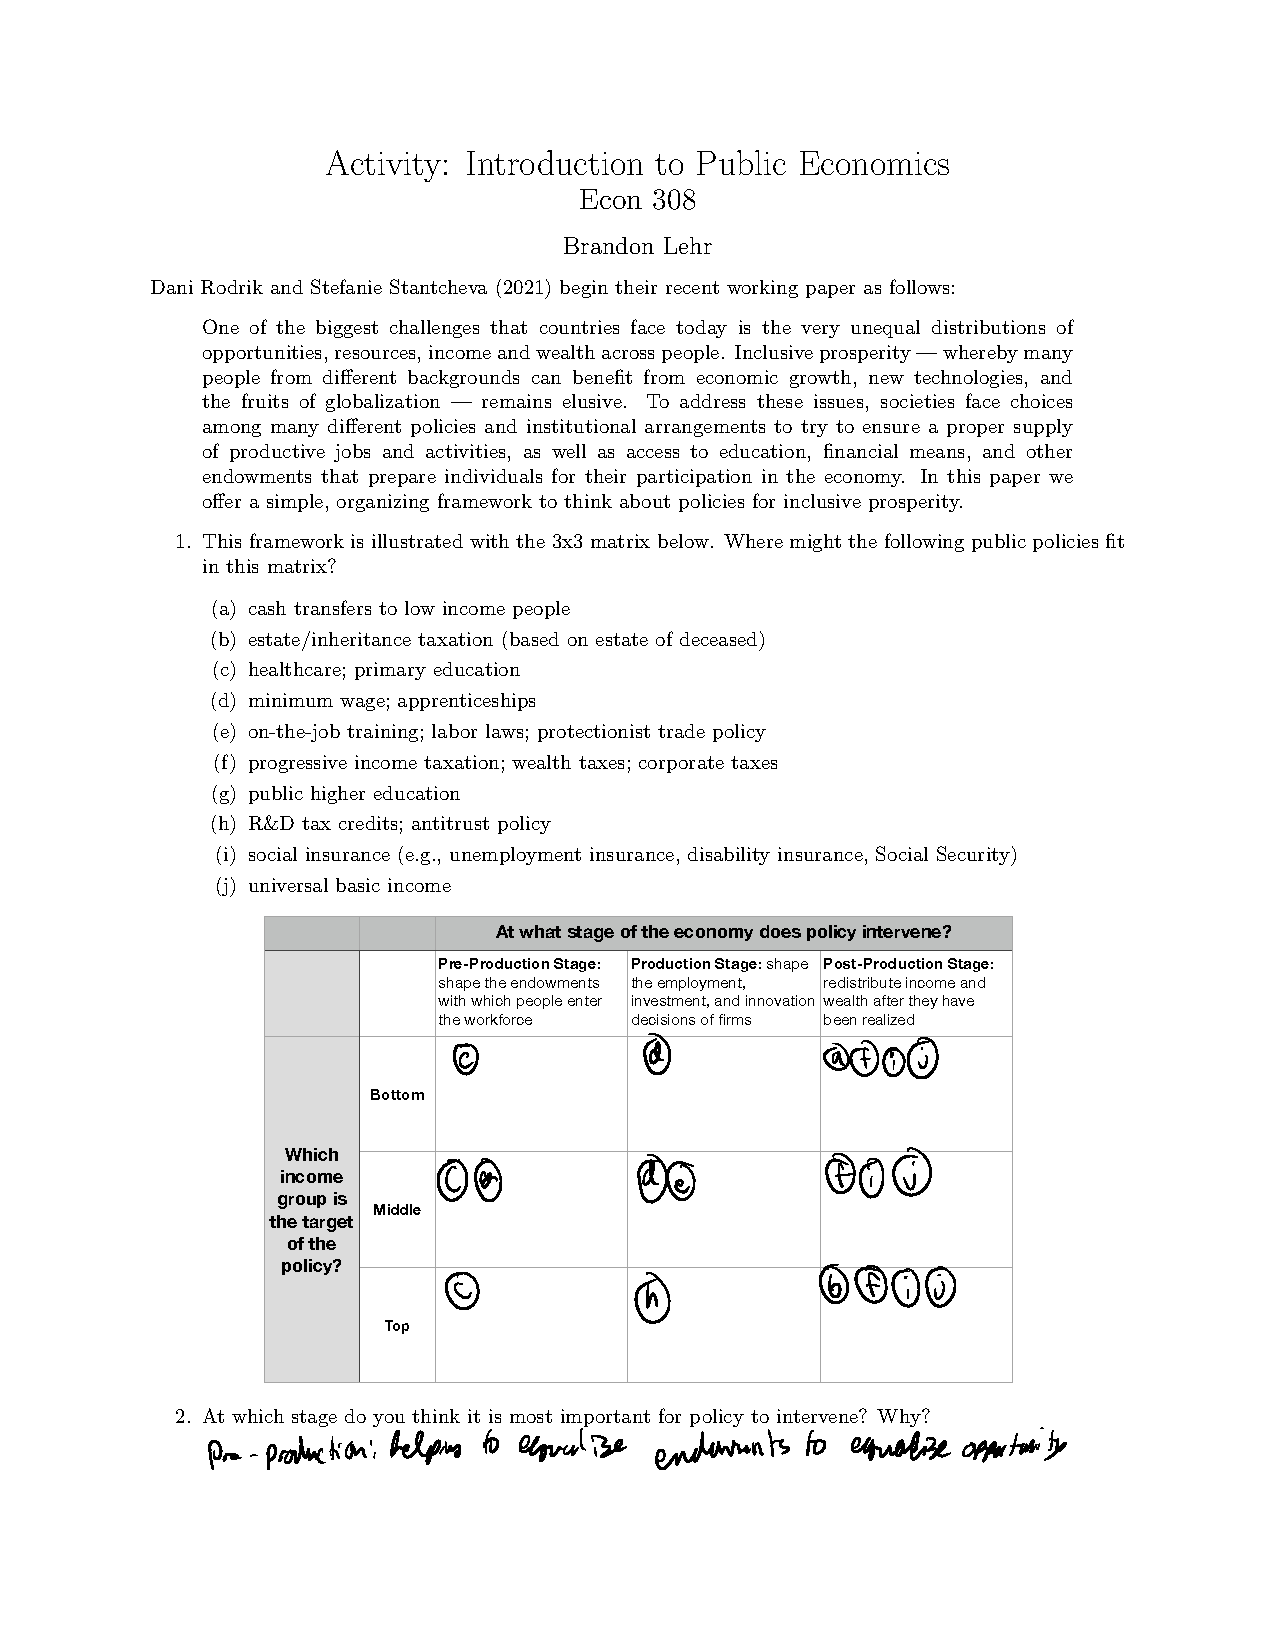
\includegraphics[width=\textwidth]{Activity_1.pdf}
      \end{center}
    \end{problem}
  \end{problem}
  \begin{problem}{Microeconomic Foundations: Consumer Theory}
    \begin{description}
      \item[Utility function] $u(X,Y)$ translates consumption quantities into utility.
      \item[Indifference curve] A graphical representation of all bundles of goods that make an individual equally well off. Mathematically, an indifference curve is the set of all bundles $(X,Y)$ such that $u(X,Y) = U$ for some utility level $U$.
      \item[Marginal Rate of Substitution] $MRS_{XY}$ is the negative slope of the indifference curve --- it's the rate at which the consumer will trade $Y$ for $X$.
        \[
          MRS_{XY} = \frac{\partial u/\partial X}{\partial u/\partial Y}
        \] 
      \item[Budget Constraint] the set of all bundles for which the total amount spent equals income
        \begin{itemize}
          \item Let $I$ indicate income and $P_X$ and $P_Y$ represent the prices of goods $X$ and $Y$ respectively.
          \item The budget constraint is the line segment $P_X X + P_Y Y = I$.
          \item The slope of the budget constraint is $-\frac{P_X}{P_Y}$.
        \end{itemize}
      \item[Utility Maximization] A rational consumer maximizes utility subject to the budget constraint via the parallel conditions of tangency ($MRS_{XY} = \frac{P_X}{P_Y}$) and the budget constraint ($P_X X + P_Y Y = I$).
      \item[Demand Functions] Utility maximization generates demand functions (quantity in terms of price) $X(P_X,P_Y,I)$ and $Y(P_X,P_Y,I)$. There are two primary canonical utility functions.
        \begin{itemize}
          \item Cobb-Douglas: $u(X,Y) = A\ln(X) + B\ln(Y)$, or $u(X,Y) = X^A \cdot Y^B$. The demand function for this utility function yields that $P_X$ has no effect on $Y$ and $P_Y$ has no effect on $X$.
          \item Quasilinear: $u(X,Y) = v(X) + BY$ where $v'(X)>0>v''(X)$ (i.e., concave down, sloping up). The demand function for this utility function yields that $I$ has no effect on $X$ assuming an interior solution.
        \end{itemize}
      \item[Price Effects] The impact of a change in $P_X$ on demand for $X$ is composed into two effects:
        \begin{itemize}
          \item Substitution Effect: change in consumption due to the change in relative prices, with utility held equal. When the price of a good increases, the substitution effect is always negative, and vice versa.
          \item Income Effect: change in consumption due to a change in purchasing power as a result of the price change, where relative prices are held constant at the final price ratio. Income effects can be positive or negative depending on the type of good.
          \item The total effect is equal to the income effect and the substitution effect.
        \end{itemize}
    \end{description}
    \begin{center}
      \begin{tcbraster}[raster columns = 1,colframe = black!75!white,colback=white,title=Income and Substitution Effects]
        \tcbincludepdf[width=10cm]{images/income_substitution.pdf}
      \end{tcbraster}
    \end{center}
    \begin{description}
      \item[Price Elasticity] The price elasticity of demand is the \% change in demand caused by a 1\% change in price of a good.
        \[
          E^D = \frac{dD}{dP}\frac{P}{D}
        \] 
      Elasticities are \textit{unit-free}, typically negative, and tend not to be constant along a demand curve.
    \end{description}
  \end{problem}
  \begin{problem}{Game Theory}
    Some decision problems involve strategic interactions between individuals.
    \begin{itemize}
      \item For example, Antonia and Bruno might care about giving to a local charity, and give $G_A$ and $G_B$ respectively. 
      \item Their utility functions depend on each other $u_A(G_A,G_B),u_B(G_A,G_B)$.
      \item The \textbf{Nash Equilibrium} yields each individual choosing an action that maximizes their utility \textit{given the other person's behavior}.
    \end{itemize}
  \end{problem}
  \begin{problem}{Social Welfare}
    Economists incorporate distributional concerns by use of social welfare functions.
    \[
      SWF = f(U_1,U_2,\dots,U_n)
    \] 
    We have two canonical social welfare functions:
    \begin{itemize}
      \item Utilitarian SWF: $SWF = U_1 + U_2 + \cdots U_n$.
      \begin{itemize}
        \item Marginal utility decreasing in income $\rightarrow$ redistribution from the rich to the poor.
        \item Taking \$1 from a rich person decreases their utility by a small amount, but transferring to a poor person increases their utility by a large amount.
      \end{itemize}
      \item Rawlsian SWF: $SWF = \min\{U_1,U_2,\dots,U_N\}$
      \begin{itemize}
        \item Social welfare is maximized by maximizing the well-being of the worst-off person.
        \item Rawlsian social welfare is more redistributive than utilitarian social welfare.
      \end{itemize}
    \end{itemize}
    There are a few other philosophies regarding the fairness of economic distribution in society.
    \begin{description}
      \item[Just deserts] Individuals should be compensated in line with their contributions.
      \item[Commodity egalitarianism] Society should ensure that individuals meet a set of basic needs, but beyond that point income distribution is irrelevant.
      \item[Equality of opportunity] Society should ensure that all individuals have equal opportunities for success.
    \end{description}
  \end{problem}
  \begin{problem}{Present Discounted Value}
    The present discounted value of a future value of money $F$ that is received and spent in $n$ periods is:
    \[
      PDV = \frac{F}{(1+r)^n}
    \] 
    For the \textbf{discount rate} $r$, typically the interest rate.\\

    For a stream of future expenses $F_i$, we use the following formula:
    \[
      PDV = \sum_{i = 1}^{n} \frac{F_i}{(1+r)^i}
    \] 
    If the values of $F_i$ are equal, then $PDV = \frac{F}{r}$, via the geometric series formula.
  \end{problem}
  \begin{problem}{Activity 2}
   \begin{tcbraster}[raster columns = 1,colframe = black!75!white,colback=white]
     \tcbincludepdf{images/Activity_2.pdf}
   \end{tcbraster} 
  \end{problem}
\end{document}
